\documentclass[polish,11pt,a4paper,twoside]{article}

\usepackage[utf8]{inputenc}
\usepackage[T1]{fontenc}
\usepackage[polish]{babel}
\usepackage[a4paper]{geometry}
\usepackage{listings}
\usepackage{graphicx}
\usepackage{amsthm}
\usepackage{color}
\usepackage{xcolor}
\usepackage{caption}
\usepackage{hyperref}
\usepackage{fancyhdr}

\definecolor{light-gray}{gray}{0.95}

\lstset {
basicstyle=\footnotesize\ttfamily,
captionpos=t,
tabsize=2,
frame=lines,
keywordstyle=\color{blue},
commentstyle=\color{gray},
stringstyle=\color{red},
breaklines=true,
showstringspaces=false,
basicstyle=\footnotesize,
emph={label},
backgroundcolor=\color{light-gray}
}
\DeclareCaptionFont{white}{\color{white}}
\DeclareCaptionFormat{listing}{\colorbox{gray}{\parbox[c][0.25cm]{\textwidth}{#1#2#3}}}
\captionsetup[lstlisting]{format=listing,labelfont=white,textfont=white}

\parskip 10.0pt
\setlength{\parindent}{0cm}

\newenvironment{items}{
\begin{itemize}
  \setlength{\itemsep}{0pt}
  \setlength{\parskip}{0pt}
  \setlength{\parsep}{0pt}
  \setlength{\topsep}{0pt}
  \setlength{\partopsep}{0pt}
}{\end{itemize}}

 \renewcommand{\familydefault}{\sfdefault}

\begin{document}

\pagestyle{fancy}
\fancyhf{} % clear all header and footer fields
\fancyfoot[R]{\footnotesize \thepage}
\renewcommand{\headrulewidth}{0pt}
\renewcommand{\footrulewidth}{0pt}

\author{Olga Zachariasz,\\Aleksander Sobol,\\Bartłomiej Bułat,\\Bartłomiej Hyży,\\Julian Król,\\Łukasz Krzyżek,\\Maciej Gąsiorski,\\Tomasz Szczęśniak\\\\Informatyka Stosowana, IV rok\\WEAIiE, AGH}
\date{30.11.2011}
\title{Zarządzanie~projektami - komunikator programistów\\Dokumentacja techniczna}
\maketitle

\tableofcontents
\pagebreak

\thispagestyle{fancy}

\section{Analiza zadania}

\subsection{Cel projektu}

Celem projektu było przygotowanie narzędzia wspierającego zdalną pracę programistów nad kodem źródłowym aplikacji.

Zadaniem naszej grupy było przygotowanie specyficznego komunikatora internetowego - przeznaczonego dla programistów. Poza typową funkcjonalnością wymiany komunikatów tekstowych, jako wymaganie postawiona została możliwość wymiany plików źródłowych, nad którymi potem przeprowadzana miała być wspólna edycja - zaznaczanie fragmentów kodu i modyfikacja istniejącego kodu. Dodatkowo komunikacja miała przebiegać pomiędzy wieloma programistami na raz, na wzór rozmów konferencyjnych znanych ze standardowych komunikatorów.

Początkowo dodatkowymi wymaganiami była implementacja rozmów głosowych oraz możliwość połączeń peer-to-peer, ostatecznie jednak wynegcjowano porzucenie tych wymagań z uwagi na dużą złożoność implementacyjną.

Aplikacja miała działać na zasadzie klient-serwer oraz wspierać dwa systemy operacyjne: Microsoft Windows (XP, 7) oraz Linux (osobna paczka dla dystrybucji Debian).

\subsection{Komunikator - use case}
% use case komunikatora

\section{Wybór technologii}

% java, smack, xmpp, jabber, istniejace serwery, itp
Jako że pozostawiono wolną rękę co do wyboru technologii, w których wykonany miał być komunikator, zespół zdecydował się na wybór bibliotek i środowisk dobrze mu znanych:
\begin{itemize}
\item Język programowania - Java
\item IDE - NetBeans
\item Protokół komunikacji - XMPP\footnote{ang. Extensible Messaging and Presence Protocol - protokół bazujący na języku XML umożliwiający przesyłanie w czasie rzeczywistym wiadomości oraz statusu; protokół ma zastosowanie nie tylko w komunikatorach, ale również w innych systemach natychmiastowej wymiany informacji (źródło: Wikipedia)}
\item Biblioteka do komunikacji przez XMPP - Smack API\footnote{Strona domowa biblioteki: http://www.igniterealtime.org/projects/smack/}
\item Biblioteka GUI - [?]
\end{itemize}

\section{Architektura komunikatora}

% klient nasz, serwer dowolny wlasciwie, rysunek
Na wybór protokołu XMPP do komunikacji pomiędzy programistami zdecydowano się głównie ze względu na jego otwartość, przystosowanie do rozszerzalności (np. o metadane informujące o edycji kodu) oraz użycie w wielu aplikacjach o podobnych możliwościach, służących do wspierania pracy grupowej zespołu programistów. Istotna okazała się również możliwość użycia istniejącej infrastruktury serwerów XMPP (dawniej Jabber), dzięki czemu wyeliminowana została konieczność implementacji programu serwera oraz dodatkowo zwiększona została niezawodność aplikacji, poprzez możliwość użycia do komunikacji dowolnego innego serwera w przypadku awarii aktualnie używanego.

Do komunikacji pomiędzy rozproszonymi klientami wybrany został serwer XMPP \emph{draugr.de}, gdyż umożliwia on niezbądne w implementowanej aplikacji rozmowy grupowe (ang. MUC - Multi User Chat) oraz rejestrację nowych kont użytkowników bezpośrednio w aplikacji, bez konieczności odwiedzania jego strony internetowej. Poglądowy schemat architektury systemu przedstawia rysunek \ref{fig:architektura}.

\begin{figure}[!htb]
  \begin{center}
    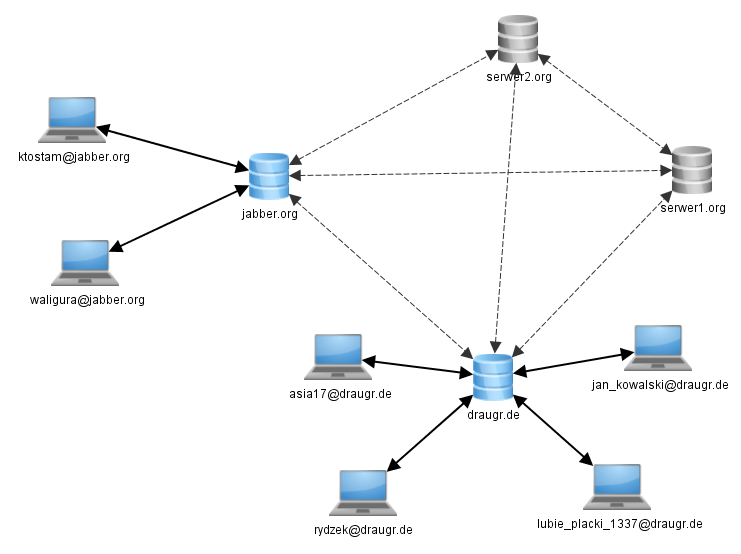
\includegraphics[width=1.0\textwidth]{img/architektura.png}
    \caption{Architektura klient-serwer komunikatora programistów} \label{fig:architektura} 
  \end{center}
\end{figure}

W aplikacji możliwe jest tworzenie nowych kont użytkowników tylko na serwerze \emph{draugr.de}, jednak możliwe jest użycie istniejącego konta z dowolnego innego serwera. Komunikacja użytkowników posiadających konta na tym samym serwerze odbywa się za pośrednictwem tego serwera. W przypadku gdy komunikacja następuje pomiędzy kontami na różnych serwerach, klient komunikatora wciąż wysyła swoje pakiety na swój serwer, zaś dopiero ten serwer przesyła go na serwer odbiorcy pakietu. Na rys. \ref{fig:architektura} liniami przerywanymi przedstawiono połączenia pomiędzy różnymi serwerami XMPP, nadzorującymi komunikację pomiędzy rozproszonymi po różnych serwerach klientami.

\section{Podział na moduły}

% klient xmpp, gui, ...?
% jest sens?

\section{Klient XMPP}

% opis co to jest, ze opakowanie smack api, itp
% schematy UML klas: XMPPClient, listener wiadomosci, itp.

\section{Komunikacja pomiędzy klientami}

\subsection{Typy komunikatów}

% zwykła wiadomosc, wiadomosc gurpowa, metadane edycji kodu, itp

\subsection{Przykład komunikacji}

% jeden klient wysyla cos do drugiego, na koncach podpiete listenery, ladny rysunek z ekranami, komunikatami, serwerami, itp

\end{document}
